\documentclass[draft]{report}   % list options between brackets

\usepackage[T1]{polski}
\usepackage[polish]{babel}
\usepackage[utf8]{inputenc}
\usepackage[dvips,pdftex,final]{graphicx}
\usepackage{rotating}
%\usepackage[T1]{fontenc}
\usepackage{fancyhdr}
%\usepackage[titles]{tocloft}
\usepackage[compact]{titlesec}
\usepackage[small]{caption}
\pagestyle{fancy}

\usepackage{geometry}
\usepackage{custom}
\usepackage{subfigure}
\usepackage{lscape}
\geometry{a4paper}

%\setlength{\cftbeforechapskip}{1.2ex}
%\setlength{\cftbeforesecskip}{0.8ex}
\titlespacing*{\section}{0pt}{0.8ex}{0.5ex}
\titlespacing{\subsection}{0ex}{0.7ex}{0.4ex}
\titlespacing{\subsubsection}{0ex}{0ex}{0ex}

%\usepackage[T1]{polski}

% type user-defined commands here

\begin{document}
\bibliographystyle{plain}

\title{<tytuł doktoratu>}
\author{Jerzy Ellert}
\date{Czerwiec 27, 2013}
\maketitle


%\begin{abstract}
%	Analiza parametrów asymetrii zmienności rytmu serca 
%\end{abstract}

\chapter*{Wstęp}

Od dość dawna, na długo przed wynalezieniem elektrokardiografu lekarze zdawali sobie
sprawę ze znaczenia badań nad rytmem serca. Jednakże przez setki lat aż do ubiegłego
stulecia generalnie jedyną techniką badawczą było osłuchiwanie. To co się nasuwało
z tych wieloletnich badań to że zmiany w rytmie serca, z uderzenia na uderzenie,
są związane z różnymi czynnikami jak np. wiek, choroba, czy ogólna kondycja
psychofizyczna pacjenta. Warto zwrócić uwagę na ogromne znaczenie badań rytmu serca w
diagnostyce medycznej Chin, także starożytnych Chin. Jednakże dokładne pomiary rytmu
serca, podlagające analizie jakościowej i ilościowej z wykorzystaniem narzędzi
matematycznych, stały się dopiero możliwe wraz z rozwojem technologicznym poczynając
od galwanometru, kimografu, wariografu pisakowego, a kończąc na cyfrowym przetwarzaniu
sygnału.

Rozwój galwanometru w XIX wieku jest związany z takimi nazwiskami jak Luigi Galvani,
Allesandro Volta, Andre-Marie Ampere, Hans Christian Oersted. Galwanometr pozwalał na
pomiar bardzo niewielkich prądów w tym biopotencjał generowany przez serce.
W 1847 roku Ludwig wynalazł kimograf z bębnem z okopconego papieru który służył
do pomiaru mechanicznej aktywności jak np ciśnienie pulsu serca. Z kolei w 1894
MacKenzie wynalazł wariograf atramentowy, a inny wynalazca, Einthoven,
połączył działanie galwanometru z możliwością wykonywania zdjęć, dzięki czemu
można było uzyskać wykresy elektrycznej aktywności serca. Natomiast rozwój
elektrokardiografu umożliwił badanie prawidłowej i nieprawidłowej elektrycznej
przewodności mięśnia sercowego.

Pierwsze udokumentowane badanie zmienności rytmu serca, u koni, przypisuje się Hale'owi
w 1733 roku. W 1847 roku Ludwig, dzięki kimografowi mógł zaobserwować, związek
pomiędzy cyklem oddechowym a zmianami częstości pulsu u psa,
co może być uznane jako pierwsza obserwacja niemiarowości oddechowej rytmu zatokowego,
w skrócie RSA (ang - Respiratory Sinus Arrhythmia). W drugiej połowie XIX wieku
podawano dwie potencjalne przyczy RSA: pierwsza, w 1865, w której Traube postawił
hipotezę, ze komórki rdzenia kręgowego kontrolujące rytm serca mogą być kontrolowane
fazowo przez bezpośrednie oddziaływanie z rdzenia przedłużonego. Współczesne
neuroanatomiczne i neurofizjologiczne badania dostarczają argumentów za współczesną
wersją tego modelu, który opiera się na generacji podstawowej częstotliwości sercowo
naczyniowej przez miedzyneuronową sieć tworzoną przez komórki rdzenia kręgowego
oraz druga zaproponowana przez Hering'a w 1871 roku który zapostulował że mechanizmem
powodującym RSA może być odruchowa regulacja sercowo-naczyniowych centrów
regulacyjnych przez sprzężenie zwrotne po pobudzeniu włókien aferentnych przez
receptory płucne. Co ciekawe, wczesne wzmianki na temat RSA można znaleść w pracach z
dziedziny psychologii, choć nie były one tak rozumiane.

W wielu publikacjach na przestrzeni lat daje się zauważyć wyrażane przez różnych
autorów znaczenie zmienności rytmu serca jako wskaźnik fizjologiczny. Wczesne prace
koncentrowały się głównie na RSA i można powiedzieć, że nie było zbyt dużego
rozróżnienia pomiędzy RSA a arytmią zatokową. Badanie nad zmiennością rytmu serca
początkowo rozwijały się w dwóch kierunkach: pierwszy koncentrował się na
zrozumieniu fizjologicznych mechanizmów wpływających na zmienność rytmu serca,
drugi był próbą znalezienia związku pomiędzy zmiennością rytmu serca a stanem
klinicznym pacjenta, ponadto można wraz z rozwojem polygrafu i jego zastosowaniem w
badaniach akademickich w latach 60-tych XX wieku wyodrębnić trzeci trend jako
poszukiwanie związków pomiędzy fizjologicznymi procesami a zmiennością rytmu serca.

Związki pomiędzy fizjologicznymi procesami a zmiennością rytmu serca można znaleść
w pracy Bainbridg'a z 1920 roku będącej próbą wyrażenia RSA w duchu zmian w
baroreceptorach i receptorach pojemnościowych w związku ze zmianami ciśnienia płucnego.
Także inni badacze jak Anrep, Pascul i Rossler zajmowali się fizjologicznymi podstawami
RSA i ich wkład jest uznawany jako pierwsze systematyczne i dogłębne studium RSA.
Trzeba także wspomnieć o pracy Hering'a z 1910 roku opisującej relacje pomiędzy
wielkością amplitudy RSA a częstotliwością pobudzenia z nerwu błednego.

Prace Eppinger'a i Hess'a z 1915 roku zapoczątkowały kliniczny aspekt badań nad
zmiennością rytmu serca i koncentrowały się na klinicznych aspektach związanych z
nieprawidłowościami w działaniu funkcji autonomicznych. Ich badania były bardzo
istotne gdyż ujawniały ważną role wegetatywnego układu nerwowego w schorzeniach
klinicznych i sugerowały związki pomiędzy tymi schorzeniami a patologiami psychicznymi,
ponadto ujawniały wrażliwość nerwu błędnego na substancje o działaniu cholinergicznym.

Zależność pomiędzy zmiennością rytmu serca a stanem systemu nerwowego była
przedmiotem badań u Wolf'a, 1967 roku, i u Hon'a, lata 1958, 1963. Hon wskazywał że
specyficzne zmiany w zmienności rytmu serca mogą być przejawem stanu zagrożenia płodu.
Z kolei Wolf wskazywał na istotne znaczenie centralnego układu nerwowego w przypadku
nagłej śmierci o podłożu kardiologicznym, w tym obszarze zmienność rytmu serca była
miernikiem komunikacji pomiędzy mózgiem, sercem a nerwem błędnym.
Należy wspomnieć, że wczesne prace ujmowały rytm serca jako zmienną zależną od
procesów kognitywnych, np. Lacey w 1967 roku, czy też procesów metabolicznych np Obrist,
1981 roku. Czasami w tym okresie zmienność rytmu serca była postrzegana jako wariancja
błędu związanego z niezbyt dokładnym aparatem pomiarowym. 

Wzrastające z czasem znaczenie zmienności rytmu serca jako interesujące zjawisko samo
w sobie oraz użycie tego fenomenu jako zmienną opisową spowodowało wyodrębnienie jej
znaczenia od konkretnych zjawiskach fizjologicznych. Wcześniejsze badanie nad zmiennością
rytmu serca odpowiadały następującym koncepcjom: (a) model oparty na indywidualnych
różnicach, traktujący zmienność rytmu serca jako zmienną charakterystyczną,
która cechuja przewidywalne wzorce zachowania iautonomiczności (np. w pracach Lacey \&
Lacey, 1958; Porges, 1972; Price, 1975; Thackray, Jones, \& Touchstone, 1975),
(b) zmienność rytmu serca jako przejaw zdrowia psychicznego (np. w pracach:
 Kahnegman, 1973; Kalsbeek \& Ettema, 1963; Lacey, 1967; Porges \& Raskin, 1969;
 Sayers, 1973), (c) kontrola zmienności rytmu serca przez oddziaływanie technikami
 biologicznego sprzężenia zwrotnego (np. w pracach Hnatiow \& Lang, 1965; Lang, Sroufe,
 \& Hastings, 1967). Oczywiście granice pomiędzy wspomnianymi koncepcjami nie zawsze są
 ostre, co z jednej strony nie ułatwia pracy badaczom, z drugiej jest ciekawym naukowym
wyzwaniem. W bardziej współczesnych badaniach wzrasta świadomość że jakość badań
ilościowych i prawidłowej interpretacji zmienności rytmu serca jest zależna nie tylko
od zrozumienia fizjologicznych procesów będących jego źródłem ale także od
związków pomiędzy tymi procesami a procesami behawioralnymi.

Historycznie można wyróżnić dwa powiązane między sobą podejścia w celu pomiaru i
ilościowej analizy zmienności rytmu serca. We wcześniejszych, szczególnie użytecznych
do badania zmienności rytmu serca płodu, stosowano krótko-okresowe tachogramy oraz
używano prostych estymatorów numerycznych np. różnica pomiędzy najkrótszym i
najdłuższym cyklem uderzeń serca. Nowsze podejścia do analizy wykorzystują bardziej
wyrafinowany aparat matematyczny - dystrybucje statystyczne (np. prace: Kleiger, Miller,
Bigger, Moss, \& Multicenter Post-Ifraction Research Group, 1987). Nowoczesne statystyczne
podejście traktuje zbiór interwałów R-R lub pary takich interwałów jako czasowo
nieuporządkowane dane i wyraża ich zmienność poprzez standardowe pojęcia statystyczne
albo poprzez geometryczne właściwości histogramów lub innych reprezentacji
geometrycznych (np Malik, 1995)

Analiza jakościowa ujawniła jedną z cech zmienności rytmu serca, mianowicie specyficzne
wzorce jakie można zaobserwować w zmienności rytmu serca daje się przyporządkować
pewnym konkretnym fizjologicznym procesom. Nowoczesne analityczne metody mające za dane
wejściowe serie interwałów R-R umożliwiły uzyskanie okresowych składowych ze wzorców
zmian w cyklach uderzeń serca oraz umożliwiły bardziej kompletną i wyrafinową
reprezentację danych, przy okazji umożliwiając zmiany w teoretycznym matematycznym
opisie tych danych. Tacy badacze jak Chess, Tam, Calaresu (1975) i Sayers (1973) do analizy
ilościowej szeregów czasowych R-R używali analizy spektralnej. Natomiast Porges i inni
do opisu związków pomiedzy zmiennością rytmu serca a oddychaniem stosowali analizę
spektrum krzyżowego i wynikiem jej zastosowania był wniosek że gestości spektralne
związane z widmem uderzeń serca mogą wyrażać oddziaływanie nerwu błędngo na serce.
Natomiast Akselrod i inni, w 1981 roku, zaproponowali następującą interpretacje
wyników analizy statystycznej: składowa rytmu oddechowego w spektrum częstotliwości
rytmu serca odpowiada oddziaływaniu nerwu błednego natomiast dwie niższe
częstotliwości reprezentują oddziaływanie pomiędzy nerwem błędnym a współczulnym
układem nerwowym. W latach 70-tych XX wieku Ewing i inni opierając się na
krótkoterminowych szeregach czasowych R-R byli w stanie określić autonomiczną
neuropatię wśród pacjentów z cukrzycą. Badania zmienności rytmu serca w późnych
latach 80-tych XX wieku także przyniosły potwierdzenie ich wartości klinicznej gdyż
stały się wyraźnym predykatorem umieralności po ostrym zawale serca. Wraz z pojawieniem
się 24 godzinnych zapisów EKG, czyli możliwością analizy długoterminowych szeregów
czasowych R-R, badacze uzyskali dodatkowe dane pomocne do określenia stratyfikacji ryzyka,
czy też ogólnie do badań stanu fizjologicznego lub patologii u pacjentów z problemami
kardiologicznymi.

Wcześniejsze podejście statystyczne do analizy zmienności rytmu serca korzystało
głównie ze statystyki opisowej jak np w pracach Lacey \& Lacey, 1958; Lang i inni, 1967;
Porges \& Raskin, 1969. Już nowsze badania datowane na lata 70-te XX wieku kładą
większy nacisk na analizę szeregów czasowych przy badaniu zmienności rytmu serca.
Zostosowanie szeregów czasowych okazało sie zasadne z dwóch powodów: pierwszy, szeregi
czasowe umożliwiły uzyskanie informacji na temat periodycznych składowych w rytmie
serca, nie bez znaczenia oraz sporej użyteczności w pracy klinicznej, drugi umożliwiły
uzyskanie wielu innych cennych informacji w dziedzinie fizjologii a także ułatwiły
modelowanie związków pomiędzy fizjologicznymi i psychicznymi procesami.


\chapter{Przegląd wybranych metod analizy HRV}

\section{Domena czasowa}

Jednym ze sposobów analizy zmienności rytmu serca są metody z zakresu domeny czasowej,
które były stosowane historycznie najwcześniej. 
Wśrod nich można wyróżnić metody
badające cały szereg odstępów $RR$, powszechnie w literaturze przedmiotu oznaczającym
odległości $R$ lub inaczej czas pomiędzy kolejnymi załamkami w elektrokardiogramie.

Wielkości określające zmienność rytmu serca w tej domenie są stosunkowo najmniej
skomplikowane. Przykładowe zmienne to: średnia wartość interwału czy różnica pomiędzy
najdłuższym i najkrótszym odcinkiem. Jednakże ze względu na niestacjonarność szeregu $RR$
w naturalny sposób pojawia się konieczność wprowadzenia bardziej skomplikowanej analizy
statystycznej, na przykład wariancja zmiennej czasowej w całym lub w części nagrania.

W domenie czasowej możemy wyróżnić także innę grupę metod zwanymi metodami geometrycznymi.
Przymiotnik geometryczny wyraża fakt użycia obiektów geometrycznych jak np:
histogram rozkładu wartości $RR$ czy wykres \PP{} którego parametry reprezentują miarę HRV. 


\subsection{Analiza pełnej zmienności HRV}

W domenie czasowej, ze względu na użyty aparat matematyczny, można wyróżnić tzw podejście
wariancyjne w którym powszechnie stosowanym parametrem jest parameter oznaczany jako
$SDNN$ będący miarą pełnej zmienności rytmu serca a wyrażony następującym wzorem:  

\begin{equation}\label{eq6}
SDNN = \sqrt{\frac{1}{n}\sum_{i=1}^{n}(RR_{i} - \overline{RR})^{2}}
\end{equation}

czyli jako pierwiastek z pełnej wariancji szeregu $RR$, gdzie $n$ jest to liczba odstępów $RR$
w całym nagraniu, $\overline{RR}$ oznacza zwykłą średnią, czyli:

\begin{equation}
\overline{RR} = \sum_{i=1}^{n}RR_{i}
\end{equation}

Nietrudno jest zauważyć że powyższe wyrażania odpowiadają drugiemu i pierwszemu momentowi
rozkładu dla szeregu odstępów $RR$. Sam w sobie szereg, wynika to także z natury
zjawiska jakim jest rytm serca, jest szeregiem niestacjonarnym w mocnym jak i słabym
sensie. Ten fakt oznacza że średnia jak i wariancja fluktuuje w czasie lub inaczej zmienia
się w zależności od tego który odcinek szeregu $RR$ analizujemy. W praktyce najcześciej
rozpatrywanymi długościami odcinka jest 5 lub 30 minut lub nagrania 24 godzinne.


\subsection{Deskryptory wykresu \PP{}}


Następna techniką z domeny czasowej wykorzystywaną do analizy HRV to technika opierająca
się na tzw. wykresach \PP{}.

Wykres \PP{}, którego nazwa pochodzi od twórcy tej techniki Henri \PP{}, jest\\ 
analityczno-wizualną technika ułatwiającą analizę złożonych zjawisk i ma ona zastosowanie
nie tylko w naukach medycznych ale także m.in. w meteorologii, geofizyce, astronomii \cite{ott}.
Element wizualny wynika z użycia odpowiednio przygotowanych wykresów i w praktyce jest to
bardzo ważny element gdyż umożliwia na bardzo szybką wstępna jakościową analizę danego
zjawiska. Element analityczny jest związany z parametrami, tak zwanymi deskryptorami,
które wyrażają ilościowo informacje zawarte w wykresie \PP{}. Należy zaznaczyć że
metod ta jest bardzo odporna na dane zawierające artefakty lub wartości odstające i w
tym sensie ma przewagę nad technikami które wymagają niezakłóconych danych np 
wykorzystujące szybką transformatę Fouriera (FFT).

Konstrukcja wykresów \PP{} jest dość prosta, przyjmując że szereg $RR$ wyrazimy jako
wektor:
\begin{equation}
\bRR = (RR_{1}, RR_{2}, \ldots, RR_{n})
\end{equation}
oś odciętych jest utworzona z wektora $RR$ bez ostatniego elementu, natomiast oś rzędnych
zawiera elementy bezpośrednio po nich następujące, czyli wektor $RR$ bez elementu
pierwszego:
\begin{equation}
\bRRm = (RR_{1}, RR_{2}, \ldots, RR_{n-1}),
\bRRn = (RR_{2}, RR_{2}, \ldots, RR_{n}) 
\end{equation}
lub inaczej
\begin{equation}
  \mathcal{P} = \{(RR_1, RR_2),\ldots, (RR_i, RR_{i+1}), (RR_{n-1}, RR_n )\},
 \label{eq:p_plot}
\end{equation}
zatem wykres \PP{} jest zbiorem (chmurą) punktów $(RR_{i}, RR_{i+1})$ gdzie $i=(1, \ldots, n-1)$

Podstawowymi parametrami (deskryptorami) utworzonymi w oparciu o powyższą reprezentacją 
graficzną wektora $\bRR$ są parametry określane w literaturze symbolami $SD1$ i $SD2$, które
wyrażają odpowiednio zmienność krótko- i długoterminową rytmu serca.
%matematycznie wyrażonymi przy pomocy wariancji:

%\begin{equation}
%SD1^2 = Var\left(\frac{\bRRn - \bRRm}{\sqrt{2}}\right)
%\end{equation}

%\begin{equation}
%SD2^2 = Var\left(\frac{\bRRn + \bRRm}{\sqrt{2}}\right)
%\end{equation}

%Tak zdefiniowane~jak powyżej
Parametry $SD1$, $SD2$ mierzą rozproszenie punktów wykresu
\PP{} względem odpowiednio tzw linii identyczności $l_{I}$ (linii dla której $\bRRm = \bRRn$)
oraz linii prostopadłej do linii identyczności $l_2$ przechodzącej przez centroid. Na
rysunku \ref{fig:pp_distrib} została przedstawiona konstrukcja tych parametrów oraz zostały
przedstawione rzuty wariancji: histogram (a) krótkoterminowej zmienności rytmu serca $SD1$
wzdłuż linii identyczności $l_{I}$, histogram (b) pełnej zmienności rytmu serca na oś $RR_n$,
histogram (c) długoterminowej zmienności rytmu serca $SD2$ wzdłuż linii prostopadłej $l_2$
do linii identyczności $l_{I}$.

Jeśli zdefiniujemy szeregi różnic i sum współrzędnych punktów obróconego PP za pomocą
relacji:


\begin{equation}
\mathbf{L_1} = \left \{ \frac{RR_1 - RR_{2}}{\sqrt{2}}, \ldots, \frac{RR_i - RR_{i+1}}{\sqrt{2}}, \ldots, \frac{RR_{n-1} - RR_{n}}{\sqrt{2}} \right \},
\end{equation}
\begin{equation}
\mathbf{L_2} = \left \{\frac{RR_1 + RR_{2}}{\sqrt{2}}, \ldots, \frac{RR_i + RR_{i+1}}{\sqrt{2}}, \ldots, \frac{RR_{n-1} + RR_{n}}{\sqrt{2}} \right \},
\end{equation}
a~sam obrót jako:
\begin{equation}
\left[
    \begin{array}{c}
      x_i\\
      y_i\\
    \end{array} \right] 
  = 
\left[ \begin{array}{c c}
      \cos(\frac{\pi}{4}) & -\sin(\frac{\pi}{4})\\
      \sin(\frac{\pi}{4}) & \cos(\frac{\pi}{4})\\
    \end{array} \right] 
\left[
    \begin{array}{c}
      \mbox{RR}_i\\
      \mbox{RR}_{i+1}\\
    \end{array} \right],
\end{equation}
to parametry $SD1$ i $SD2$ możemy wyrazić jako wariancje szeregów $\mathbf{L_1}$ i $\mathbf{L_2}$ \cite{poinc_jaro,jarek2}:
\begin{equation}
  SD1^2 = \mbox{Var}( \mathbf{L_1})
  = \mbox{Var}\left(\frac{\bRRn - \bRRp}{\sqrt{2}}\right),
  \label{eq:sd1}
\end{equation}
\begin{equation}
  SD2^2 = \mbox{Var}( \mathbf{L_2})
  = \mbox{Var}\left(\frac{\bRRn + \bRRp}{\sqrt{2}}\right). 
  \label{eq:sd2}
\end{equation}

\begin{figure}
\centering
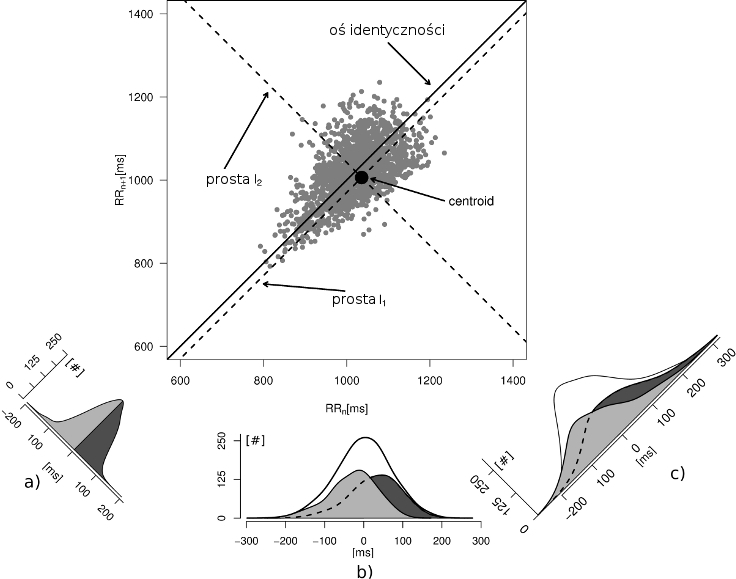
\includegraphics[width=\textwidth]{graph/pp_distrib.jpg}
\caption{Rysunek prezentuje położenie prostej równoległej ($l_1$) i~prostej prostopodłej ($l_2$) do osi identyczności separującej punkty reprezentujące skrócenia i~wydłużenia odstępów $RR$. Na wykresie przedstawiono również rozkłady punktów opisujących zmienność krótkoterminową $SD1$ (panel $a$ - rzut PP na oś $l_2$), zmienność długoterminową $SD2$ (panel $c$ reprezentujący rzut PP na oś $l_1$) oraz zmieność całkowitą (panel $b$ -- rzut PP na oś odciętych). Na histogramach różnymi odcieniami szarości oznaczono wkłady pochodzące od punktów, znajdujących się nad i~pod osią identyczności. Opracowano na podstawie \cite{hrstruct} -- rysunek udostępniony przez Jarosława Piskorskiego i~Przemysława Guzika na licencji CC BY.}
\label{fig:pp_distrib}
\end{figure}

Poniżej jeszcze inna postać na wariancje $SD1$ i $SD2$ tym razem oparta na własnościach geometrycznych linii identyczności występującej na rysunku \ref{fig:pp_distrib}: 

\begin{equation}
SD1^2 = \frac{1}{n}\sum_{i=1}^{n}r_{i}^{\perp 2}
\end{equation}

\begin{equation}
SD2^2 = \frac{1}{n}\sum_{i=1}^{n}r_{i}^{\parallel 2}
\end{equation}

gdzie $r_{i}^{\perp}$ jest prostopadłą odległością punktu $(RR_{i}, RR_{i+1})$ do linii
identyczności, $r_{i}^{\parallel}$ jest odległością punktu $(RR_{i}, RR_{i+1})$ do linii
$l_2$ wzdłuż linii identyczności.

Należy zaznaczyć że wyrażenie (\ref{eq:sd1}) dla krótkoterminowej zmienności rytmu serca
nie jest z matematycznego punktu widzenia odchyleniem standardowym, gdyż nie jest
wyznaczane względem linii $l_1$ przechodzącej przez centroid, to znaczy nie minimalizuje
drugiego momentu rozkładu punktów $RR$. Jednakże to w żaden sposób
nie umniejsza użyteczności tego deskryptora i to z dwóch powodów: (1) linia
identyczności dzieli cały wykres \PP{} na dwie części, górną dotyczącą zwolnień,
dolną dotyczącą przyspieszeń, zatem $SD1$ liczona względem $l_{I}$ ma wyraźną interpretację
fizjologiczną, (2) różnica pomiędzy wariancjami odnoszącymi się odpowiednio do linii $l_1$
oraz $l_{I}$ zgodnie z wartościami podanymi w \cite{poinc_jaro} jest rzędu $10^{-5}$ i
dąży do $0$ dla coraz większej liczby pomiarów, ponadto sam błąd związany z wprowadzeniem
wariancji względem $l_{I}$ jest rzędu $10^{-8}$, zatem w praktyce jest zaniedbywalny.

Relacja pomiędzy krótkoterminową i długoterminową zmiennością rytmu serca opisanymi powyżej
a miarą pełnej zmienności rytmu serca opisanej w \ref{subsec:pelna_zmiennosc}
jest następująca:
\begin{equation}
SDNN^2 = \frac{1}{2}(SD1^2 + SD2^2)\label{SDNNpartitioning}.
\end{equation}

\subsection{Deskryptory asymetrii rytmu serca}

Opierając się między innymi na analizie szeregów czasowych $RR$ przy pomocy wykresów \PP{}
grupa badaczy z Katedry i Kliniki Intensywnej Terapii Kadriologicznej i Chorób Wewnętrznych
Uniwersytetu Medycznego im. Karola Marcinkowskiego w Poznaniu oraz Instytutu Fizyki
Uniwersytetu Zielonogórskiego odkryła nowe zjawisko fizjologiczne w zmienności rytmu serca
nazwane asymetrią rytmu serca. Słowo asymetria wyraża interesujące fenomen polegający na
tym, że wkład zwolnień rytmu serca w zmienności krótkoterminowej jest większy niż wkład
przyspieszeń, natomiast w zmienności długoterminowej i całkowitej odwrotnie, wkład
przyspieszeń jest większy niż wkład zwolnień.

Elementem geometrycznym względem którego ta asymetria jest określana została przedstawiona
w rozdziale (UZUEPLNIC) jako linia identyczności (rysunek \ref{fig:pp_distrib}). Linia identyczności jest jedyną linią posiadającą jasną interpretację fizjologiczną, dzieląca
rytm serca na grupy zwolnień i przyspieszeń.

Opierając się na właściwościach matematycznych wariancji można dokonać podziału wszystkich
parametrów wykresu \PP{}, tzn $SD1^2$, $SD2^2$ i $SDNN^2$, na części dotyczące zwolnień i 
przyspieszeń.

\subsubsection{Deskryptory asymetrii krótkoterminowej}
Podział $SD1^2$ dla przyspieszeń i zwolnień wygląda następująco:
\begin{equation}
SD1^2=\frac{1}{n}\left(\sum_{i=1}^{n_{d}}[r^{\perp\;d}_{i}]^{2}+\sum_{j=1}^{n_{a}}[r^{\perp\;a}_{j}]^{2}\right),\label{SD1_podzial}
\end{equation}
gdzie:
\begin{enumerate}
\item[]$r^{\perp\;d}_{i}$ -- odległość prostopadła przyspieszającego punktu  wykresu \linebreak \PP{} o~indeksie $i$ do linii identyczności,
\item[]$r^{\perp\;a}_{j}$ -- odległość prostopadła zwalniającego punktu wykresu \PP\ o~indeksie $j$ do linii identyczności.
\end{enumerate}
oraz
\begin{enumerate}
\item[]$n_{d}$ -- jest liczbą zwolnień (punktów powyżej linii identyczności),
\item[]$n_{a}$ -- jest liczbą przyspieszeń (punktów poniżej linii identyczności).
\end{enumerate}
Faktycznie występuje jeszcze trzecia grupa punktów leżąca na linii identyczności, a zatem
$n$ będąca całkowitą ilością punktów bedzię zdefiniowana jako:
\begin{equation}
n=n_{d}+n_{a}+n_{on} \label{nki},
\end{equation}
jednakże punkty $n_{on}$ nie wnoszą żadnego wkładu do $SD1$, dlatego można je tutaj pominąć.

Wyrażenie (\ref{SD1_podzial}) składa się dwóch członów które w~naturalny sposób odpowiadają
wkładom zwolnień i~przyspieszeń w całkowitej $SD1^{2}$ 
\begin{equation}
SD1^{2}=SD1_{d}^{2}+SD1_{a}^{2}\label{SD1par},
\end{equation}
gdzie
\begin{equation}
SD1_{d}^{2}=\frac{1}{n}\sum_{i=1}^{n_{d}}[r^{\perp\;d}_{i}]^{2}, \qquad SD1_{a}^{2}=\frac{1}{n}\sum_{i=1}^{n_{a}}[r^{\perp\;a}_{i}]^{2}. \label{STpart}
\end{equation}
Do analizy porównawczej wariancje określone przez wzory (\ref{STpart}) użyte z danymi
pochodzącymi od różnych osób nie są zbyt pomocne, dlatego zostały wprowadzone wielkości
wyrażające znormalizowane wkłady zwolnień i przyspieszeń (UZUPELNIC BIBLIO), tzn.:
\begin{equation}
C1_{d}=\frac{SD1_{d}^{2}}{SD1^{2}}, \qquad C1_{a}=\frac{SD1_{a}^{2}}{SD1^{2}},\label{STnorm}
\end{equation}
przy czym
\begin{equation}
C1_{d}+C1_{a}=1.
\end{equation}

\subsubsection{Deskryptory asymetrii długoterminowej}

Długoterminowa zmienność rytmu serca, $SD2$, obliczana jako wariancja względem linii
centroidu $l_2$ (rysunek \ref{fig:pp_distrib}), w przeciwieństwie do $SD1$, jest
najmniejszym możliwym drugim momentem w tym kierunku. Ponieważ, linia identyczności jest
jedyną linią z jasną interpretacją fizjologiczną to konstrukcja deskryptorów asymetrii dla
$SD2$ jest definiowana względem tej linii, natomiast linia $l_2$ prostopadła do linii
identyczności jest używana tylko do obliczeń.

Podział $SD2^2$ dla przyspieszeń i zwolnień jest koncepcyjnie bardzo podobny do wyrażenia
(\ref{SD1_podzial}), a mianowicie
\begin{equation}
SD2^2= \frac{1}{n}\sum_{s=1}^{n}r^{||\;2}_{s}=\frac{1}{n}\left(\sum_{i=1}^{n_{d}}[r^{||\;d}_{i}]^{2}+\sum_{j=1}^{n_{a}}[r^{||\;a}_{j}]^{2}+\sum_{k=1}^{n_{on}}[r^{||\;on}_{k}]^{2}\right), \label{LTpart}
\end{equation}
gdzie:  
\begin{enumerate}
\item[]$r^{||}_{s}$ -- odległością punktu \emph{s} od $l_{2}$ wzdłuż linii identyczności,
\item[]$n_{d}$, $n_{a}$ i~$n_{on}$ -- są tak samo definiowane jak dla wzoru (\ref{SD1_podzial}), 
\item[]$r^{||\;d}_{i}$ -- odległość mierzona wzdłuż linii identyczności zwalniającego punktu  wykresu \PP\ o~indeksie $i$ do linii $l_{2}$,
\item[]$r^{||\;a}_{j}$ -- odległość mierzona wzdłuż linii identyczności przyspieszającego punktu  wykresu \PP\ o~indeksie $j$ do linii $l_{2}$.
\end{enumerate}
Podobnie jak w przypadku zmienności krótkoterminej, dwa pierwsze człony we wzorze (\ref{LTpart})
odpowiadają zwolnieniom i przyspieszeniom rytmu serca, jednakże to co odróżnia zmienność
długoterminową to niezaniedbywalny człon zawierający punkty na linii identyczności, czyli:
$1/n\sum_{k=1}^{n_{on}}[r^{||\;on}_{k}]^{2}$ w~(\ref{LTpart}). Wielkość członu związanego
z linią identyczności jest, jeśli tak można wyrazić, zależna sprzętowo, gdyż na ilość 
identycznych (co do wartości) sąsiadujących ze sobą punktów w szeregu $RR$ istotny wpływ ma
precyzja urządzenia pomiarowego. Czym większa precyzja, tym mniej punktów pomiarowych
wpada do tego samego przedziału pomiędzy dwoma dyskretnymi poziomami pomiarowymi, a to
znaczy dążenie do zera liczby punktów na linii identyczności. 

W pracy (UZUPELNIC BIBLIO) zaproponowano aby człon związany z linią identyczności miał
równy wkład, po połowie, do obu części zwolnień i przyspieszeń, i wielkości tak określone
okazują się bardziej konserwatywne, jak to pokazały testy statystyczne.
 
Podział asymetryczny dla zmienności długoterminowej $SD2$ definiuje się analogicznie jak w 
 (\ref{SD1par}), tzn.:
\begin{equation}
SD2^{2}=SD2_{d}^{2}+SD2_{a}^{2}, \label{SD2part}
\end{equation}
czyli na część pochodzącą od zwolnień i przyspieszeń, a odpowiednie wkłady do wariancji
(UZUPELNIC BIBLIO) przy pomocy następujących wyrażeń:
\begin{eqnarray}
SD2_{d}^{2}&=&\frac{1}{n}\left(\sum_{i=1}^{n_{d}}[r^{||\;d}_{i}]^{2}+\frac{1}{2}\sum_{j=1}^{n_{on}}[r^{||\;on}_{j}]^{2}\right),\label{LTpartdef}\\
SD2_{a}^{2}&=&\frac{1}{n}\left(\sum_{i=1}^{n_{a}}[r^{||\;a}_{i}]^{2}+\frac{1}{2}\sum_{j=1}^{n_{on}}[r^{||\;on}_{j}]^{2}\right). \nonumber
\end{eqnarray}

Uwaga związana ze znormalizowanymi wkładami zwolnień i przyspieszeń przy okazji wzoru (\ref{STnorm})
obowiązuje także dla zmienności długoterminowej, co wyrażają następujące relacje:
\begin{equation}
C2_{d}=\frac{SD2_{d}^{2}}{SD2^{2}}, \qquad C2_{a}=\frac{SD2_{a}^{2}}{SD2^{2}},\label{LTnorm}
\end{equation}
gdzie
\begin{equation}
C2_{d}+C2_{a}=1.
\end{equation}

\subsubsection{Deskryptory asymetrii pełnej}
Opierając się na deskrytorach asymetrii krótko- i długoterminej można dokonać podziału
pełnej zmienności rytmu serca, wzór (\ref{SDNNpartitioning}), na składowe dla zwolnień i
przyspieszeń w następujący sposób (UZUPELNIC BIBLIO)
\begin{eqnarray}
SDNN^{2}&=&\frac{1}{2}\left(\underbrace{(SD1_{d}^{2}+SD1_{a}^{2})}_{SD1^{2}}+\underbrace{(SD2_{d}^{2}+SD2_{a}^{2})}_{SD2^{2}}\right)\\
&=&\frac{1}{2}\left(\underbrace{(SD1_{d}^{2}+SD2_{d}^{2})}_{2SDNN_{d}^{2}}+\underbrace{(SD1_{a}^{2}+SD2_{a}^{2})}_{2 SDNN_{a}^{2}}\right).\nonumber
\end{eqnarray}
lub inaczej jako
\begin{equation}
SDNN^{2}=SDNN_{d}^{2}+SDNN_{a}^{2}, \label{SDNNpart}
\end{equation}
przy czym 
\begin{equation}
SDNN_{d}^2=\frac{1}{2}\left(SD1_{d}^{2}+SD2_{d}^{2}\right),\quad SDNN_{a}^2=\frac{1}{2}\left(SD1_{a}^{2}+SD2_{a}^{2}\right). \label{SDNNpartad}
\end{equation}

Wyrażenie (\ref{SDNNpartad}) w naturalny sposób umożliwia zdefiniowanie	znormalizowanych
wkładów zwolnień i przyspieszeń do pełnej zmienności rytmu serca (UZUPELNIC BIBLIO)
\begin{equation}
C_{d}= \frac{SDNN_{d}^{2}}{SDNN^{2}},\qquad C_{a}= \frac{SDNN_{a}^{2}}{SDNN^{2}}\label{SDNNcontrib}.
\end{equation}
przy czym
\begin{equation}
C_{d}+C_{a}=1.
\end{equation}

Proces konstruowania deskryptorów asymetrii krótko- i długoterminowej jest zobrazowany na
rysunku~\ref{habfig2_2}{.}
Zgodnie z analizą przeprowadzoną w (BIBLIO) asymetria krótkoterminowa w grupie $N$
badanych osób zachodzi w stopniu istotnym statystyczne, jeśli: 
\begin{equation}
C1_{d}>C1_{a},
\end{equation} 
Natomiast asymetria długoterminowa zachodzi w stopniu istotnym statystycznie, jeśli:
\begin{equation}
C2_{d}<C2_{a},
\end{equation}
oraz asymetria całkowita jest określona gdy w~grupie $N$ badanych osób, jeśli jest
spełniona poniższej nierówność w stopniu istotny statystycznie (BIBLIO) %\cite{annals}.
\begin{equation}
C_{d}<C_{a}.
\end{equation}
Wielkość próby oraz szczegóły metod statystycznych użytych w celu określenia zachodzenia
powyższych warunków zostały podane w pracy (BIBLIO).

\subsubsection{Aplikacje kliniczne deskryptorów asymetrii}

Opierając się na danych klinicznych, jak to zostało pokazane w pracach (BIBLIO), 
potwierdzono występowanie asymetrii krótkoterminowej w szeregach odstępów $RR$ u osób 
zdrowych w spoczynku i to w stopniu wysoce istotnie statystycznym. Podobnie, asymetria
długoterminowa została potwierdzona w grupie osób zdrowych w spoczynku w stopniu wysoce
istotnie statystycznym, w pracach (BIBLIO). Także w tych pracach została potwierdzona
asymetria rytmu serca względem pełnej zmienności rytmu serca, $SDNN^2$, w stopniu wysoce
istotnie statystycznym. Natomiast w pracach (BIBLIO) można znaleść kliniczne aplikacje
wariancyjnych parametrów asymetrii rytmu serca.

Ponieważ opisane w tym rozdziale deskrytory asymetrii są ze swojej natury pojęciami
całkowicie ogólnymi, mogą być użyte także do badanie asymetrii innych zjawisk medycznych.
I tak, w pracy (BIBLIO), jest badana (i potwierdzona) asymetria krótkoterminowa w zmienności
sygnału ciśnienia tętniczego. Stwierdzono, że jest ona niezależna od HRA.
%\linebreak %przeniesienie związane ze składem
\begin{landscape}
\begin{figure}
\begin{center}
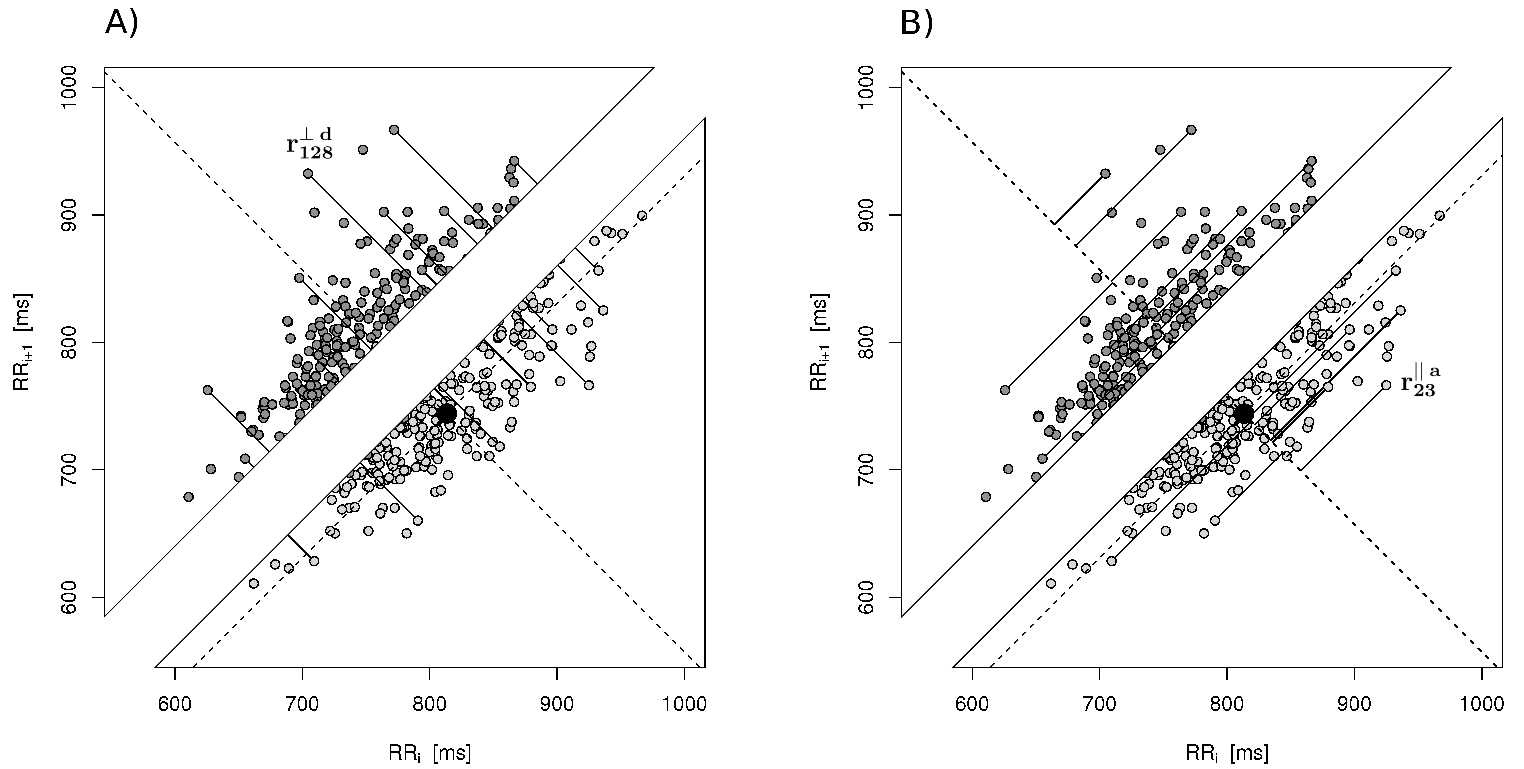
\includegraphics[width=1.5\textwidth]{graph/habfig2_2a}
\caption{W panelu A) przedstawiono konstrukcję deskryptorów krótkoterminowej HRA, a~w~panelu B) proces konstrukcji deskryptorów długoterminowej HRA. Należy zwrócić uwagę, że linia identyczności jest najistotniejszym obiektem geometrycznym w~obu konstrukcjach -- jest ona jedynym kryterium decydującym o~tym, czy dany punkt wnosi wkład do części wariancji ($SD1^2$, $SD2^2$ lub $SDNN^2$) związanej ze zwolnieniami czy przyspieszeniami. $r^{\perp\;d}_{128}$ jest prostopadłą odległością (zwalniającego) punktu wykresu \PP{} numer $128$ do linii identyczności, $r^{||\;a}_{23}$ jest prostopadłą odległością (przyspieszającego) punktu numer $23$ od linii $l_{2}$.\label{habfig2_2}}
\end{center}
\end{figure}
\end{landscape}
\clearpage

\section{Domena częstotliwości - analiza spektralna}

Drugą grupą technik wykorzystywanych do analizy rytmu serca jest analiza
spektralna. Należy zaznaczyć że większa część teoretycznego opisu HRV wywodzi
się właśnie z zastosowania takiego rodzaju technik \cite{task2, hrv_origins, dynamicMalik}. 
W analizie spektralnej, podobnie jak w domenie czasowej, jest brana pod uwagę wariancja
lecz stosuje się inne nazewnictwo oraz troche inny język matematyczny.
Mianowicie wariancja przy podejściu spektralnym nazywana jest mocą spektralną, która jest 
wyliczana w podziale na częstotliwości z badanego zakresu, przy czym podział zakresu
częstotliwości jest dokonywany trochę sztucznie bez silnego związku z fizjologią. Podział
zakresu pasma dla krótkich nagrań, rzędu 2-5 minut, zwykłe przebiega następująco: (a) 
zakres 0,15 - 0,4 Hz wysoka częstotliwość, (b) zakres 0,04 - 0,15 Hz niska częstotliwość, (c)
poniżej 0,04 bardzo niska częstotliwość, dodatkowo (d) zakres poniżej 0,003 Hz,
występujący w przypadku dłuższych nagrań np. 24 godzinnych, zwany ultraniską częstotliwością.
Przyjmuje się że wplywy układu współczulnego oraz oddychania \cite{task2, hrv_origins, dynamicMalik, Hainsworth} są reprezentowane przez widmo w zakresie wysokich częstotliwości; na widmo z
zakresu niskich częstotliwości wpływają oba podukłady autonomicznego układu nerwowego; 
natomiast dla widma z pozostałych zakresów tzn bardzo niskich i ultra niskich częstotliwości
nie jest znany, w obecnym stanie wiedzy, związek z fizjologią w kontekście HRV. 

Wykorzystywana w analizie spektralnej funkcja gęstości spektralnej jest obliczana wprost i
można tego dokonać w dwojaki sposób: z wykorzystaniem metod nieparametrycznych albo przy
pomocy estymujących metod parametrycznych dla których wymagane jest przyjęcie $a\:priori$
pewnego modulu matematycznego opisującego sygnał wejściowy uzyskany z szeregu $RR$ a
wynikiem tej estymacji jest periodogram \cite{task2, hrv_origins, shumway, lomb_o, scargle, lombCasti, dsp_engel}. Wyznaczanie wariancji odpowiadającej pasmu
częstotliwości dokonuje się przy pomocy całkowania po częstotliwościach związanych z tym
pasmem. 

W praktyce, wśród metod nieparametrycznych szczególnym uznaniem i zastosowaniem cieszy się
metoda zwana szybką transformatą Fouriera (ang. Fast Fourier Transform, FFT). Wsród metod
parametrycznych najpopularniejsza jest metoda autoregresyjna wykorzystująca do estymacji
wielomian, czego konsekwencją jest to że nie wszystkie dane są ujęte w periodogramie, tym
niemniej ciągle jest możliwe wnioskowanie statystyczne \cite{task, hrv_origins, dsp_engel, lomb,scargle,lombCasti,shumway}. Cechą wspólną obu metod jest
konieczność użycia resamplingu lub inaczej interpolacji tachogramu przez równomierne w
czasie próbkowanie a także potrzeba interpolacji 'zakłóceń' tzn. uderzeń ektopowych oraz
artefaktów. Resampling tachogramu zwykle wykonuje z częstością co 250 ms.

Jednym z większych problemów przy analizie spektralnej szeregu czasowego $RR$ jest jego
niestacjonarność. Objawia się to między innymi tym że skład widmowy spektralnej funkcji
gęstości nie odpowiada oscylacjom w systemie sercowo-naczyniowym, na przykład daje się
zaoobserwować duży wkład powolnych trędów czy też brzegowych własności szeregu czasowego
w widmie niskich częstotliwości. Próbą poradzenia sobie z tymi problemami jest użycie metod
pozwalających na niwelowanie niestacjonarności czy też gwałtownym zmianom fazy, jednakże
jest to związane z niepożądaną zmianą struktury szeregu czasowego. W związku z tym wydaje
się zasadne użycie innych specjalistycznych metod oscylacyjnych, przykłady można znaleść
w pracach \cite{task2, hrv_origins, prsa_k}.     
 
Parametry analizy spektralnej jako takie bardzo różnią się pomiędzy osobami, zatem w celu
umożliwienia ich porównywania stosuje się tak zwane znormalizowane parametry analizy
spektralnej, LFnu oraz HFnu, wyrażone przez następujące relacje:
\begin{equation}
\mathrm{HFnu=\frac{HF}{HF+LF}},\qquad \mathrm{LFnu=\frac{LF}{HF+LF}}. \label{HFLFnu}
\end{equation}
gdzie: HF - moc widma szeregu $RR$ w zakresie wysokich częstotliwości 0,15-0,4 Hz;
LF - moc widma szeregu $RR$ w zakresie niskich częstotliwości 0,04-0,15 Hz.

\subsection{Transformata Fouriera}

W ogólnym zarysie transformata Foriera polega na rozkładzie sygnału na szereg funkcji
sinusidalnych z odpowiednio dobranymi aplitudami i częstotliwościami. Istnieją cztery typy
transformat \cite{dsp} które dzielą się ze względu na: (a) zachowanie sygnału - periodyczny,
aperiodyczny; (b) typ sygnału - ciągły, dyskretny. Wspólną ich cechą jest to że
zawsze operują na sygnałach nieskończonych, zatem sygnał uzyskany z ograniczonego w czasie
szeregu $RR$ nie jest poprawnym, z formalnego punktu widzenia, źródłem danych dla
transformaty Fouriera. Najcześciej tą niedogodność rozwiązuje się na dwa sposoby:
(a) przyjmuje się wartości zero z lewej i prawej strony sygnału, zatem uzyskuje się sygnał
dyskretny aperiodyczny; lub (b) zakłada się występowania kopii sygnału z lewej i prawej jego
strony, zatem uzyskuje się sygnał dyskretny periodyczny. Z powodów praktycznych
lepsze do obliczeń numerycznych jest podejścia (b) gdyż nie ma problemu z koniecznością
reprezentowania aperiodycznego sygnału przez nieskończoną liczbę sinusoid, czyli w tym
przypadku stosuje się tzw dyskretną transformatę Fouriera (ang. DFT - Discrete Fourier
Transform). Działanie DFT na $N$-elementowy dyskretny sygnał czasowy generuje dwa $N/2+1$
elementowe szeregi amplitud $C$ oraz $S$ dla funkcji \emph{cosinus} oraz \emph{sinus}, co
wyraża następująca relacja:

\begin{equation}
  x[i] = \sum_{k=0}^{N/2} \bar{C}[k]\cos( \frac{2\pi k i}{N}) + \sum_{k=0}^{N/2}\bar{S}[k]\sin( \frac{2\pi k i}{N})
  \label{eq:dft}
\end{equation}
gdzie $x$ to szereg z domeny czasowej, $\bar{C}[k] = \frac{C[k]}{N/2}$, $\bar{S}[k] = -\frac{S[k]}{N/2}$, $\bar{C}[0] = \frac{C[0]}{N}$, $\bar{C}[N/2] = \frac{C[N/2]}{N}$ a $i=[0,\ldots,N]$. Indeks $k$ reprezentuje
częstotliwości funkcji \emph{cosinus} oraz \emph{sinus}, a $C[k]$ i $S[k]$ opisują
amplitudę, przypadającą na daną częstotliwość. Postać wzoru (\ref{eq:dft}) określa także
sposób przejścia (syntezy) sygnału z domeny częstotliwości do domeny czasowej.
Jadnakże należy zwrócić uwagę na bardzo ważny fakt związany z analizą szeregów czasowych
$RR$. Pełna transformata Fouriera zawiera dwa człony:
amplitudowe widmo mocy które odpowiada wariancji z domeny czasowej oraz widmo fazowe
które nie jest rozpatrywane w obszarze HRV. Fakt odrzucania członu fazowego powoduje że
nie można przejść z domeny częstotliwości do domeny czasowej i dotyczy to specyficznie
szeregów czasowych $RR$, a nie ogólnych matematycznych rozważań w kontekście relacji (\ref{eq:dft}). 
Powyższe zdanie można wyrazić obrazowo w ten sposób: nie jest możliwe odtworzenie kształtu
szeregu $RR$, w szczególności serii zwolnień i przyspieszeń, wychodząc z domeny
częstotliwości do domeny czasowej z powodu 'zgubienia' widma fazowego w transformacie
Fouriera.

Użycie DFT do analizy spektralnej HRV, wymaga aby wejściowy sygnał bedący szeregiem odstępów
$RR$ przedstawić w postaci tachogramu o równoodległych punktach \cite{splines}. Tachogram jest następnie
interpolowany oraz wygładzany przy pomocy odpowiedniego filtra np typu \emph{boxcar} \cite{boxcar}.

Spośród kilku metod przy pomocy których można wykonać analizę spektralną DFT,
algorytm szybkiej transformaty Fouriera (ang. fast Fourier transform, FFT) \cite{cooleyfft} cieszy się
największym uznaniem z powodu najlepszej wydajności obliczeniowej.

\subsection{Periodogram Lomba}

Wśród metod parametrycznych możemy wyróżnić metodę będącą rozwinięciem analizy spektralnej,
znaną pod nazwą periodogramu Lomba-Scargle'a (LSP). Szczególna użyteczność tej metody
polega między innymi na tym że nie wymaga resamplingu, tak jak wcześniej wspomniana 
metoda autoregresyjna. Jest ona realizowana przy pomocy metody najmniejszych kwadratów.
Ze względu na brak resamplingu nie jest konieczne aby szereg czasowy, np. $RR$, miał stałą
częstość próbkowania, zatem można użyć bezpośrednio oryginalnych danych [UZUPELNIC BIBLIOGRAFIE],
a wszelkie pobudzenia ektopowe, zwane inaczej pobudzeniami przeniesionymi oraz
artefakty techniczne nie wpływają na poprawność działania periodogramu Lomba-Scargle'a.

Pochodna powyższej metody o nazwie uśrednionego periodogramu Lomba-Scargle'a została
opracowana w trakcie eksperymentu w którym osoby biorące w nim udział miały za zadanie
oddychać z zadaną częstotliwością. W eksperymencie badacze weryfikowali
hipotezę czy istnieje sprzężenie mechaniczne pomiędzy czynnością układu sercowo-naczyniowego
a oddechem o określonym rytmie. 

Technicznie metoda uśrednionego periodogramu Lomba-Scargle'a (ALSP) wykorzystuje uśredniony i
znormalizowany periodogram Lomba-Scargle'a dla badanej populacji szeregów. Wyrażanie
definiujące znormalizowany periodogram z odjętą średnią dla jednego szeregu z populacji
jest następujące:

\begin{eqnarray}
P_{X}(f)&=&\frac{1}{2SDNN^{2}}\left\{\frac{\left[ \sum_{i=1}^{n}(RR(t_{i})-\overline{RR})\cos(2\pi f(t_{i}-\tau))\right]^{2}}{\sum_{i=1}^{n}\cos^{2}(2\pi f(t_{i}-\tau))}\right. \label{LSPeriodogram}\nonumber\\ 
&+&\left. \frac{\left[ \sum_{i=1}^{n}(RR(t_{i})-\overline{RR})\sin(2\pi f(t_{i}-\tau))\right]^{2}}{\sum_{i=1}^{n}\sin^{2}(2\pi f(t_{i}-\tau))}\right\}
\label{eq:lomb} ,
\end{eqnarray}
gdzie $n$ jest długością szeregu czasowego, wyrażoną w~punktach, a~nie w~czasie,
$\overline{RR}$ jest jego średnią, $SDNN^{2}$ jego wariancją, a~$\tau(t)$ jest zależnym od
częstości przesunięciem fazowym sprawiającym, że periodogram jest niezmienniczy względem
przesunięć w czasie \cite{c++,thong,lomb,vanicek}:
\begin{equation}
\tan(4\pi f\tau)=\frac{\sum_{i=1}^{n}\sin(4\pi f t_{i})}{\sum_{j=1}^{n}\cos(4\pi f t_{j})}. \label{tau}
\end{equation}
gdzie $t_{i}$ to punkty ścieżki czasu szeregu $RR$ (sumy kumulatywnej szeregu $RR$, tj.
zbioru $\{t_0=RR_0, t_1=RR_0+RR_1, t_2=RR_0+RR_1+RR_2, \ldots, \sum_{i=0}^n RR_i \}$)
odpowiadające poszczególnym odstępom $RR$ w~następujący sposób
\begin{equation}
RR(t_{i})\equiv RR_{i}\equiv t_{i}-t_{i-1}, \label{RRy}
\end{equation}
czyli $t_{i}$ odpowiada pozycji kompleksu QRS o~numerze $i+1$.

Powyższa metoda jest szczególnie użyteczna jeśli stosujemy ją dla różnych szeregów
czasowych $RR$ pochodzących od różnych osób w celu wyodrębnienia wspólnych częstotliwości,
i nie jest, jak napisano wcześniej, stosowany resampling. W literaturze można znaleść m.in
następujące dwa opisy efektywności metod (LSP/ALSP): (a) w artykule \cite{laguna} autorzy 
stosują LSP wyznaczając widmo szeregu $RR$ ze szczególnym naciskiem na zmienną szerokość próbkowania oraz przerwy w sygnale wynikające z usuwania pobudzeń ektopowych; (b) w pracy
\cite{thong} stosują ALSP dla okien czasowych o stałej szerokości z tego
samego szeregu $RR$. Opisywana tutaj metoda ALSP dla różnych szeregów z różnych źródeł
jest technicznie bardzo podobna do tej z \cite{thong} jednakże ich własności matematyczne
oraz zakres interpretacji znacznie się różni. Pierwsza podstawowa różnica polega na sposobie
denormalizacji periodogramu w którym zamiast pełnej wariancji $SDNN^2$ jak w definicji
(\ref{eq:lomb}) stosuje się fragment pasma częstotliowościowego który można fizjologicznie
zinterpretować i wariancję oblicza się w zakresie 0.04 - 0.4 Hz, $SDNN^2$ zostaje zastąpione
przez poniższe wyrażenie:
\begin{equation}
  \sigma = \sum_{f\in[0.04,0.4Hz]}A_f^2,
\end{equation}
gdzie $A_f^2$ jest amplitudą sinusoidy o~częstotliwości $f$. Druga różnica to końcowe
uśrednianie po grupie szeregów pochodzących od różnych osób, czyli:
\begin{equation}
  \overline{P_{X}(f)} = \frac{1}{M}\sum_{k=1}^{M}P_{X}^k(f),
  \label{eq:alsp}
\end{equation}
gdzie $M$ jest liczbą analizowanych szeregów a $P_{X}^k(f)$ jest periodogramem
Lomba-Scargle'a dla $k$-tego szeregu. Podsumowując, uśredniony LSP można zinterpretować
jako średni wkład pasma częstotliwościowego w zadanym zakresie widma 0.04 - 0.4 Hz.
Wszystkie częstotliwości które przejawiają podobne zachowanie w sensie spektralnym w 
indywidualnych szeregach danej grupy badanych osób będą wzmacniane w wyniku uśredniania.
Podobieństwo zachowania spektralnego częstości polega na spójnie wysokim lub niskim
wkładzie w całkowitej wariancji lub mocy. Jeśli zachodzi sytuacja odwrotna, to znaczy wkład
częstości w całkowitej mocy ulega zmianie z nagrania na nagranie wtedy następuje wygaszanie
tychże częstości w wyniku uśrednienia.

%\section{Introduction 2}     % section 1.1
%\subsection{History 2}       % subsection 1.1.1

%\chapter{\LaTeX}           % chapter 2
%\section{Introduction}     % section 2.1
%\subsection{Usage}         % subsection 2.1.1

%\begin{thebibliography}{9}
  % type bibliography here
%\end{thebibliography}

\bibliography{literatura}


\end{document}